Für spätere Rechnungen werden die bauteilspezifischen Werte notiert.
\begin{align*}
  R &= \SI{48,1\pm0,1}{\Omega}\\
  C &= \SI{2,098\pm0,006}{nF}\\
  L &= \SI{10,00\pm0,03}{mH}
\end{align*}
\\Mit der in Abbildung \ref{aufbau1} dargestellten Schaltung wird die Amplitudenabnahme eines RCL-Schwingkreises ermittelt.
 \begin{figure}[h!]
   \centering
   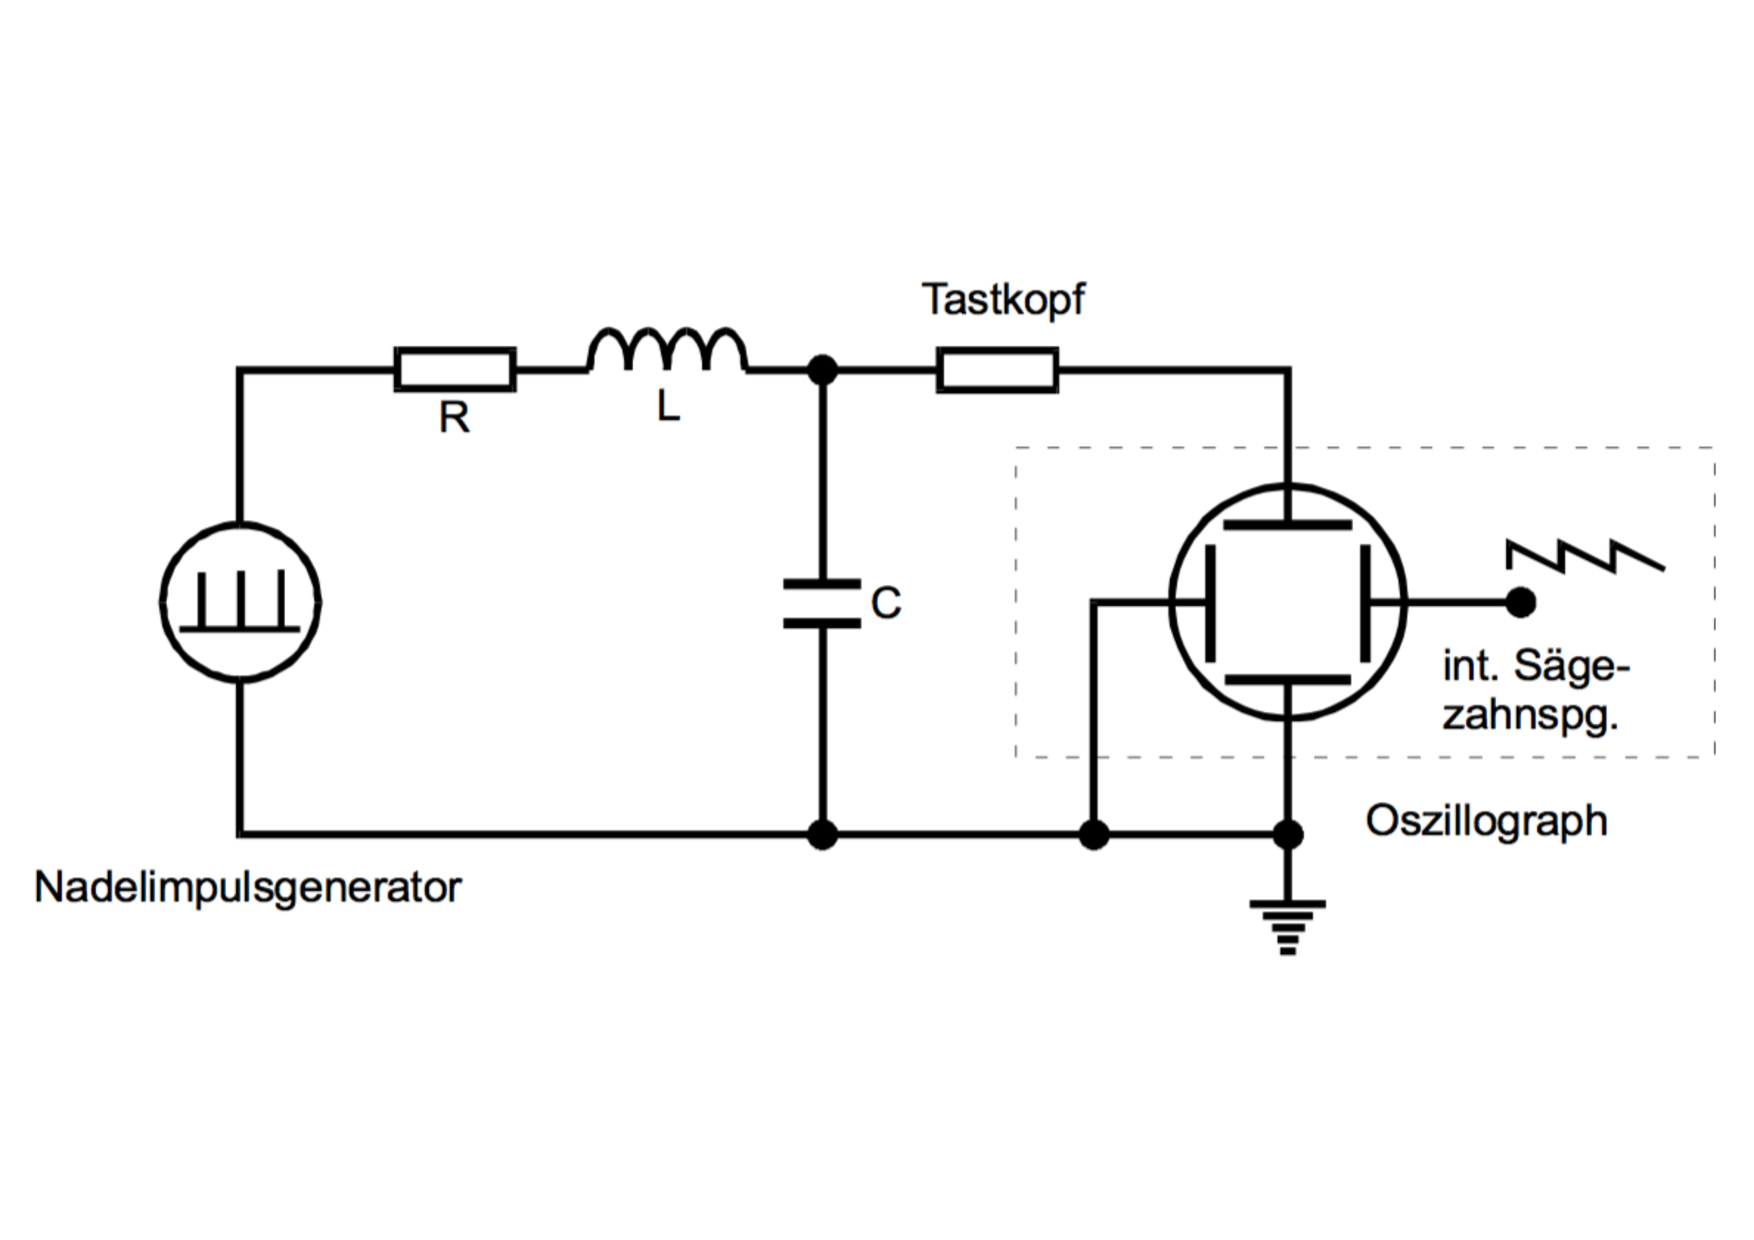
\includegraphics[width=\textwidth]{aufbau1.pdf}
   \caption{Schaltung zur Untersuchung der Zeitabhängigkeit der Amplitude einer gedämpften Schwingung \cite{1}}
   \label{aufbau1}
 \end{figure}
 \\Daraus lässt sich die Abklingdauer $T_{ex}$ und der Dämpfungswiderstand $R_{eff}$ bestimmen.
Am Oszilloskop wird die Spannung gegen die Zeit aufgetragen und Wertepaare entnommen.
Im angefertigten Thermodruck wird die einhüllende e-Funktion hinzugefügt.\\

Nun wird der Widerstand für den aperiodischen Grenzfall ermittelt.
Dazu wird der Widerstand durch ein Potentiometer ersetzt. Der Widerstand wird nun so variiert das sich ein Graph ergibt, der eben keine Überschwingungen besitzt.
Der zugehörige Wert für $R_{ap}$ wird notiert.
Mit dem Versuchsaufbau aus der Abbildung \ref{aufbau2} wird die Frequenzabhängigkeit der Kondensatorspannung untersucht.
\newpage
\begin{figure}[h!]
  \centering
  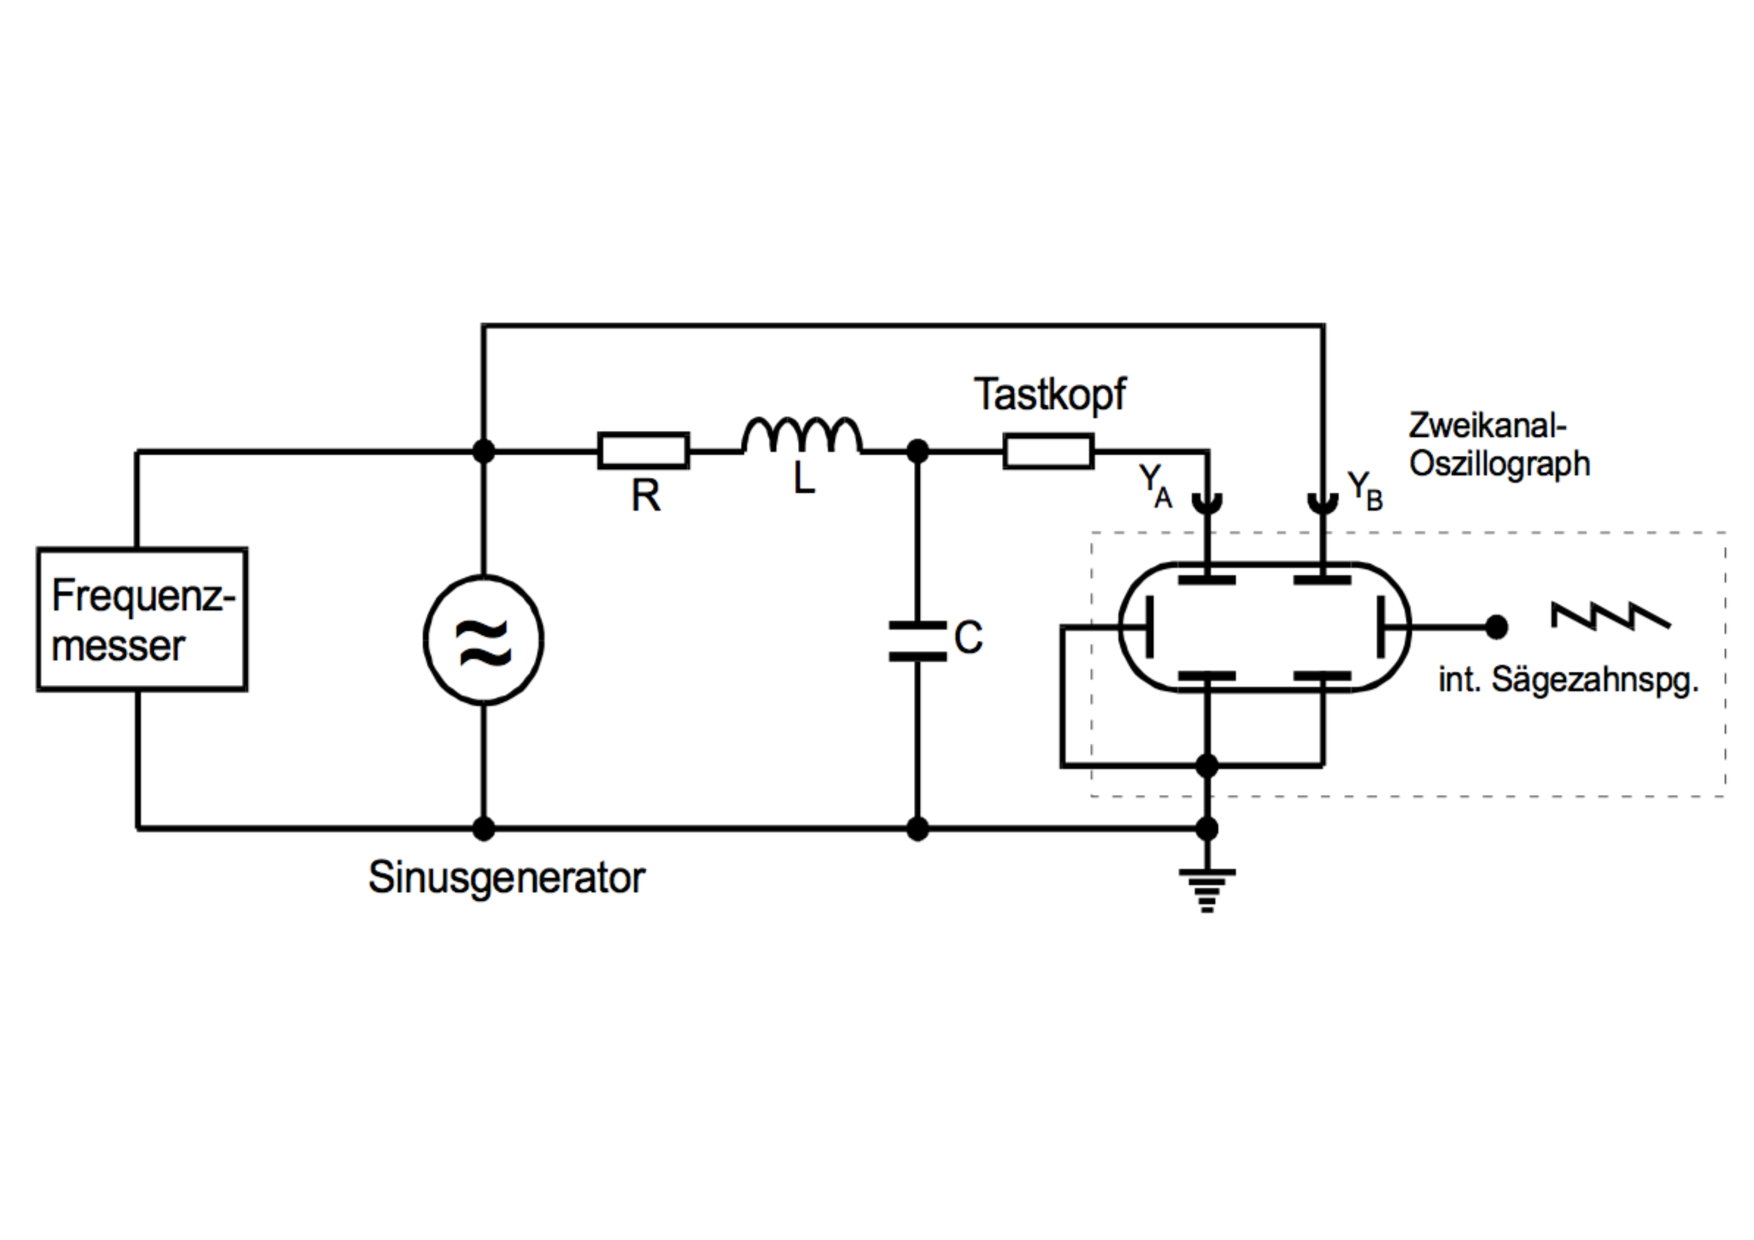
\includegraphics[width=\textwidth]{aufbau2.pdf}
  \caption{Schaltung zur Messung der Frequenzabhängigkeit der Phase Zwischen Erreger- und Kondensatorspannung bei einem RLC-Kreis \cite{1}}
  \label{aufbau2}
\end{figure}
Als erstes wird die Erregerspanung $U_{0}$ ermittelt. Anschließend wird am Sinusgenerator die Frequenz \nu verändert und die dazu gehörige Spannung gemessen.\\

Im letzten Versuchsteil wird in Abhängigkeit von der Frequenz \nu die Phasenverschiebung \varphi zwischen der Kondensatorspannung $U_c$ und der Erregerspannung $U_{0}$ gemessen.
Wie in der Abbildung \ref{phasenverschiebung} zu sehen werden die Werte für a und b gemessen.
\begin{figure}[h!]
  \centering
  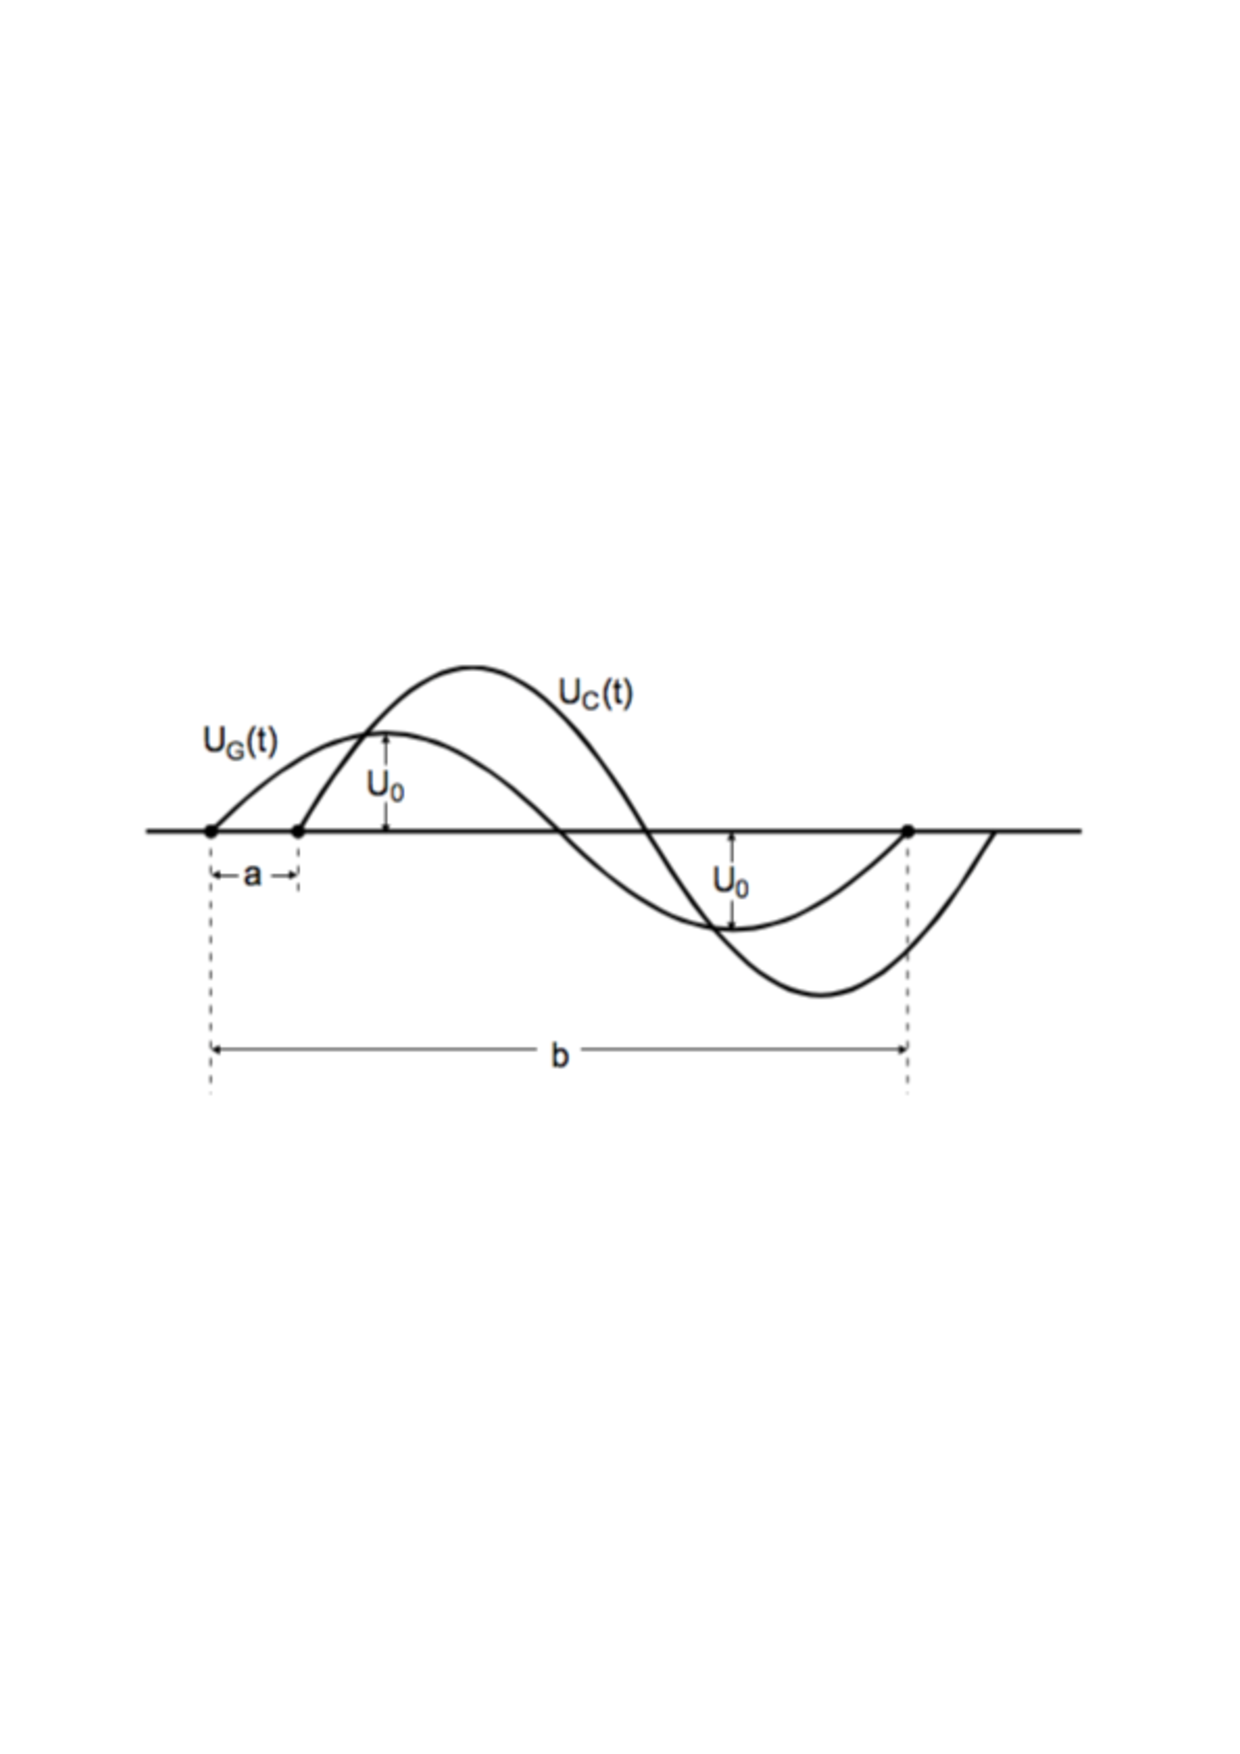
\includegraphics[width=\textwidth]{phasenverschiebung.pdf}
  \caption{Phasenverschiebung \cite{2}}
  \label{phasenverschiebung}
\end{figure}
